\chapter*{\large\textsf{Linda und Gordon bedanken sich}}
        \thispagestyle{empty}

Vielen Dank allen Beteiligten! Eigentlich ist da vor allem Doris zu danken, die hat lektoriert. Sie übernimmt dadurch die Verantwortung für \emph{alle} Rechtschreibfehler, grammatikalischen Fehlgriffe, schiefe Formulierungen, Schachtelsätze und andere Übeltäter.

Aber auch allen unbekannten Software-Entwicklern, die die Umsetzung des Buches indirekt erst ermöglicht haben. Gesetzt wurde das Dokument in \LaTeX, die Brotschrift ist \emph{Quattrocento} von Pablo Impallari, siehe auch www.impallari.com. Die Überschriften sind in \emph{French Cursive} von Emmanuel Beffara (http://beffara.org/stuff/frcursive) gesetzt. Es wurden sehr viele Pakete eingebunden, die nicht alle aufgezählt werden sollen. Die \LaTeX-Quelldateien befinden sich alle auf https://github.com/GordonWiegand/tina. Die Datei binder.pdf ist das Buch als PDF. In binder.tex sind alle verwendeten Pakete aufgeführt, jeweils mit kurzem Kommentar versehen, was die machen.


Zum Bearbeiten (Ausschneiden) der Bilder kam Inkscape zum Einsatz. Auch das Titelbild wurde mit Hilfe von Inkscape erstellt. 
        \thispagestyle{empty}

Auf der folgenden und letzten Seite gibt es als grafischen Abschluss noch ein Ausmalbild. Das ist tatsächlich zum ausmalen gedacht! Also Buntstifte raus und los geht es! Und nicht vergessen ein Foto davon an uns zu schicken!

\afterpage{
    \begin{figure}
        \thispagestyle{empty}    
        \centering
        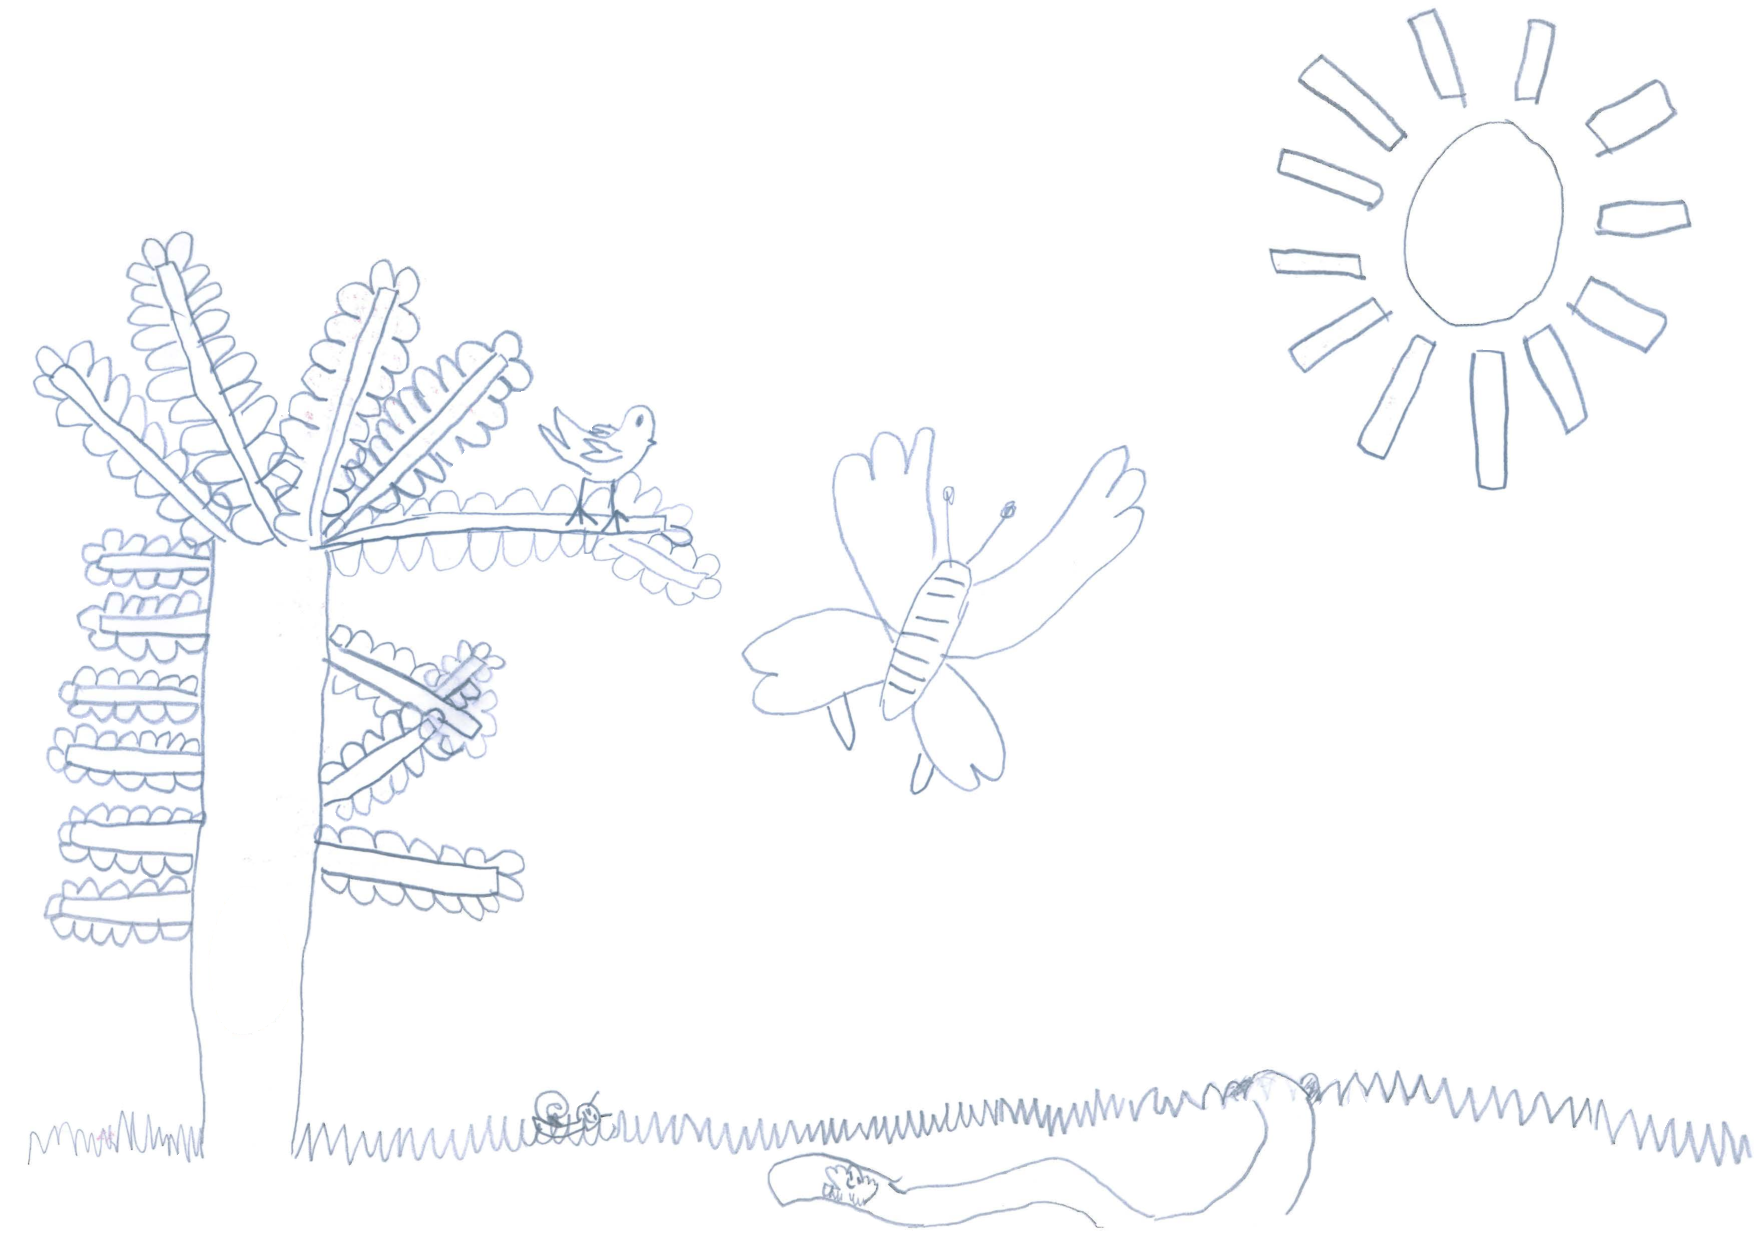
\includegraphics[height=\textwidth,angle=90]{bilder/ausmalbild.pdf}
    \end{figure}
    \clearpage
}

